\documentclass[]{article}
\usepackage{lmodern}
\usepackage{amssymb,amsmath}
\usepackage{ifxetex,ifluatex}
\usepackage{fixltx2e} % provides \textsubscript
\ifnum 0\ifxetex 1\fi\ifluatex 1\fi=0 % if pdftex
  \usepackage[T1]{fontenc}
  \usepackage[utf8]{inputenc}
\else % if luatex or xelatex
  \ifxetex
    \usepackage{mathspec}
  \else
    \usepackage{fontspec}
  \fi
  \defaultfontfeatures{Ligatures=TeX,Scale=MatchLowercase}
\fi
% use upquote if available, for straight quotes in verbatim environments
\IfFileExists{upquote.sty}{\usepackage{upquote}}{}
% use microtype if available
\IfFileExists{microtype.sty}{%
\usepackage{microtype}
\UseMicrotypeSet[protrusion]{basicmath} % disable protrusion for tt fonts
}{}
\usepackage[margin=1in]{geometry}
\usepackage{hyperref}
\hypersetup{unicode=true,
            pdfborder={0 0 0},
            breaklinks=true}
\urlstyle{same}  % don't use monospace font for urls
\usepackage{longtable,booktabs}
\usepackage{graphicx,grffile}
\makeatletter
\def\maxwidth{\ifdim\Gin@nat@width>\linewidth\linewidth\else\Gin@nat@width\fi}
\def\maxheight{\ifdim\Gin@nat@height>\textheight\textheight\else\Gin@nat@height\fi}
\makeatother
% Scale images if necessary, so that they will not overflow the page
% margins by default, and it is still possible to overwrite the defaults
% using explicit options in \includegraphics[width, height, ...]{}
\setkeys{Gin}{width=\maxwidth,height=\maxheight,keepaspectratio}
\IfFileExists{parskip.sty}{%
\usepackage{parskip}
}{% else
\setlength{\parindent}{0pt}
\setlength{\parskip}{6pt plus 2pt minus 1pt}
}
\setlength{\emergencystretch}{3em}  % prevent overfull lines
\providecommand{\tightlist}{%
  \setlength{\itemsep}{0pt}\setlength{\parskip}{0pt}}
\setcounter{secnumdepth}{0}
% Redefines (sub)paragraphs to behave more like sections
\ifx\paragraph\undefined\else
\let\oldparagraph\paragraph
\renewcommand{\paragraph}[1]{\oldparagraph{#1}\mbox{}}
\fi
\ifx\subparagraph\undefined\else
\let\oldsubparagraph\subparagraph
\renewcommand{\subparagraph}[1]{\oldsubparagraph{#1}\mbox{}}
\fi

%%% Use protect on footnotes to avoid problems with footnotes in titles
\let\rmarkdownfootnote\footnote%
\def\footnote{\protect\rmarkdownfootnote}

%%% Change title format to be more compact
\usepackage{titling}

% Create subtitle command for use in maketitle
\newcommand{\subtitle}[1]{
  \posttitle{
    \begin{center}\large#1\end{center}
    }
}

\setlength{\droptitle}{-2em}

  \title{}
    \pretitle{\vspace{\droptitle}}
  \posttitle{}
    \author{}
    \preauthor{}\postauthor{}
    \date{}
    \predate{}\postdate{}
  

\begin{document}

\hypertarget{mendelian-genetics}{%
\section{Mendelian Genetics}\label{mendelian-genetics}}

In this laboratory session, we will use maize \emph{Zea mays} subsp.
mays, from Spanish: maíz after Taíno mahiz), also known as corn to study
\href{https://en.wikipedia.org/wiki/Mendelian_inheritance}{Mendelian
inheritance}. This cereal grain was first domesticated by indigenous
peoples in southern Mexico about 10,000 years ago. The leafy stalk of
the plant produces separate pollen and ovuliferous inflorescences or
ears, which are fruits, yielding kernels or seeds. Maize has become a
staple food in many parts of the world, with total production surpassing
that of wheat or rice. However, not all of this maize is consumed
directly by humans. Some of the maize production is used for corn
ethanol, animal feed and other maize products, such as corn starch and
corn syrup. The six major types of corn are dent corn, flint corn, pod
corn, popcorn, flour corn, and sweet corn.

The principles of Mendelian inheritance were named for and first derived
by \href{https://en.wikipedia.org/wiki/Gregor_Mendel}{Gregor Johann
Mendel}, a nineteenth-century Moravian monk who formulated his ideas
after conducting simple hybridisation experiments with pea plants
(\emph{Pisum sativum}) he had planted in the garden of his monastery.
Between 1856 and 1863, Mendel cultivated and tested some 5,000 pea
plants. From these experiments, he induced two generalizations which
later became known as Mendel's Principles of Heredity or Mendelian
inheritance (Table @ref(tab:mendel)). He described these principles in a
two-part paper, Versuche über Pflanzen-Hybriden (Experiments on Plant
Hybridization), that he read to the Natural History Society of Brno on 8
February and 8 March 1865, and which was published in 1866. Mendel's
conclusions were largely ignored by the vast majority of scientists at
the time. In 1900, however, his work was ``re-discovered'' by three
European scientists, Hugo de Vries, Carl Correns, and Erich von
Tschermak.

Mendel discovered that, when he crossed purebred white flower and purple
flower pea plants (the parental or P generation), the result was not a
blend. Rather than being a mix of the two, the offspring (known as the
F1 generation) was purple-flowered. When Mendel self-fertilized the F1
generation pea plants, he obtained a purple flower to white flower ratio
in the F2 generation of 3 to 1. In the first experiment, we will examine
the F2 generation resulting from the F1 generation obtained from a
parental generation of yellow and purple corn.

He then conceived the idea of heredity units, which he called
``factors''. Mendel found that there are alternative forms of
factors---now called genes---that account for variations in inherited
characteristics. For example, the gene for flower color in pea plants
exists in two forms, one for purple and the other for white. The
alternative ``forms'' are now called alleles. For each biological trait,
an organism inherits two alleles, one from each parent. These alleles
may be the same or different. An organism that has two identical alleles
for a gene is said to be homozygous for that gene (and is called a
homozygote). An organism that has two different alleles for a gene is
said be heterozygous for that gene (and is called a heterozygote).

Mendel hypothesized that allele pairs separate randomly, or segregate,
from each other during the production of gametes: egg and sperm. Because
allele pairs separate during gamete production, a sperm or egg carries
only one allele for each inherited trait. When sperm and egg unite at
fertilization, each contributes its allele, restoring the paired
condition in the offspring. This is called the Law of Segregation.
Mendel also found that each pair of alleles segregates independently of
the other pairs of alleles during gamete formation. This is known as the
Law of Independent Assortment. In the second experiment, we will observe
this law exemplified by a dihybrid cross of corn.

The genotype of an individual is made up of the many alleles it
possesses. An individual's physical appearance, or phenotype, is
determined by its alleles as well as by its environment. The presence of
an allele does not mean that the trait will be expressed in the
individual that possesses it. If the two alleles of an inherited pair
differ (the heterozygous condition), then one determines the organism's
appearance and is called the dominant allele; the other has no
noticeable effect on the organism's appearance and is called the
recessive allele. Thus, in the example above the dominant purple flower
allele will hide the phenotypic effects of the recessive white flower
allele. This is known as the Law of Dominance but it is not a
transmission law: it concerns the expression of the genotype. The upper
case letters are used to represent dominant alleles whereas the
lowercase letters are used to represent recessive alleles.

\begin{longtable}[]{@{}ll@{}}
\caption{(\#tab:mendel) Mendel's laws of inheritance.}\tabularnewline
\toprule
\begin{minipage}[b]{0.22\columnwidth}\raggedright
Law\strut
\end{minipage} & \begin{minipage}[b]{0.72\columnwidth}\raggedright
Definition\strut
\end{minipage}\tabularnewline
\midrule
\endfirsthead
\toprule
\begin{minipage}[b]{0.22\columnwidth}\raggedright
Law\strut
\end{minipage} & \begin{minipage}[b]{0.72\columnwidth}\raggedright
Definition\strut
\end{minipage}\tabularnewline
\midrule
\endhead
\begin{minipage}[t]{0.22\columnwidth}\raggedright
Law of segregation\strut
\end{minipage} & \begin{minipage}[t]{0.72\columnwidth}\raggedright
During gamete formation, the alleles for each gene segregate from each
other so that each gamete carries only one allele for each gene.\strut
\end{minipage}\tabularnewline
\begin{minipage}[t]{0.22\columnwidth}\raggedright
Law of independent assortment\strut
\end{minipage} & \begin{minipage}[t]{0.72\columnwidth}\raggedright
Genes for different traits can segregate independently during the
formation of gametes.\strut
\end{minipage}\tabularnewline
\begin{minipage}[t]{0.22\columnwidth}\raggedright
Law of dominance\strut
\end{minipage} & \begin{minipage}[t]{0.72\columnwidth}\raggedright
Some alleles are dominant while others are recessive; an organism with
at least one dominant allele will display the effect of the dominant
allele.\strut
\end{minipage}\tabularnewline
\bottomrule
\end{longtable}

\hypertarget{punnett-square}{%
\subsection{Punnett square}\label{punnett-square}}

The \href{https://en.wikipedia.org/wiki/Punnett_square}{Punnett square}
(Figures @ref(fig:punnett) and @ref(fig:punnettF1)) is a visual
representation of Mendelian inheritance and used to predict an outcome
of a particular cross or breeding experiment. It is named after
\href{https://en.wikipedia.org/wiki/Reginald_Punnett}{Reginald C.
Punnett}, who devised the approach. In our first experiment, both
parents are homozygous, one carrying two copies of the dominant allele
(R), the other two copies of the recessive (r) allele. Each parent can
only make gametes that have either the R (purple) or r (yellow) allele.
The Punnett square for the parental cross is shown in Figure
@ref(fig:punnett)

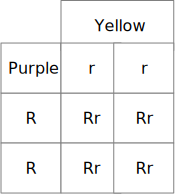
\includegraphics{./figures/mendel/Punnett.svg} The squares containing
the single letters represent the possible gametes. The squares with two
letters represent the zygotes resulting from the combination of the
respective gametes. It can be easily seen that all offspring will be
heterozygous (Rr) and therefore purple. The Punnett square for the F1
cross is depicted in Figure @ref(fig:punnettF1)

\begin{figure}
\centering
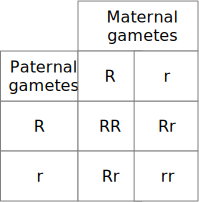
\includegraphics{./figures/mendel/PunnettF1.svg}
\caption{Punnett square for heterozygous cross.}
\end{figure}

\hypertarget{test-cross}{%
\subsection{Test cross}\label{test-cross}}

A \href{https://en.wikipedia.org/wiki/Test_cross}{test cross}, first
introduced by Gregor Mendel, involves the breeding of an individual with
a phenotypically recessive individual, in order to determine the
zygosity of the former by analyzing proportions of offspring phenotypes.
Zygosity can either be heterozygous or homozygous. Those that are
heterozygous have one dominant and one recessive allele. Individuals
that are homozygous dominant have two dominant alleles, and those that
are homozygous recessive have two recessive alleles.

The genotype that an offspring has for each of its genes is determined
by the alleles inherited from its parents. The combination of alleles is
a result of the maternal and paternal chromosomes contributed from each
gamete at fertilization of that offspring. During meiosis in gametes,
homologous chromosomes experience genetic recombination and segregate
randomly into haploid daughter cells, each with a unique combination of
maternally and paternally coded genes. Dominant alleles will override
the expression of recessive alleles.

Test crosses are used to test an individual's genotype by crossing it
with an individual of a known genotype. Individuals that show the
recessive phenotype are known to have a homozygous recessive genotype.
Individuals that show the dominant phenotype, however, may either be
homozygous dominant or heterozygous. The phenotypically dominant
organism is the individual in question in a test cross. The purpose of a
test cross is to determine if this individual is homozygous dominant or
heterozygous.

Test crosses involve breeding the individual in question with another
individual that expresses a recessive version of the same trait.
Analyzing the proportions of dominant and recessive offspring determines
if the individual in question is homozygous dominant or heterozygous. If
all offspring from the test cross display the dominant phenotype, the
individual in question is homozygous dominant; if half the offspring
display dominant phenotypes and half display recessive phenotypes, then
the individual is heterozygous. Since the homozygous recessive
individual can only pass on recessive alleles, the alleles the
individual in question passes on determine the phenotypes of the
offspring.

\hypertarget{monohybrid-cross-experiment-1}{%
\subsection{Monohybrid cross (Experiment
1)}\label{monohybrid-cross-experiment-1}}

A \href{https://en.wikipedia.org/wiki/Monohybrid_cross}{monohybrid
cross} is a mating between two individuals with different variations at
one genetic trait of interest. The character(s) being studied in a
monohybrid cross are governed by two or multiple variations for a single
locus. A cross between two parents possessing a pair of contrasting
characters is known as monohybrid cross. To carry out such a cross, each
parent is chosen to be homozygous or true breeding for a given trait
(locus). When a cross satisfies the conditions for a monohybrid cross,
it is usually detected by a characteristic distribution of
second-generation (F2) offspring that is sometimes called the monohybrid
ratio.

Generally, the monohybrid cross is used to determine the dominance
relationship between two alleles. The cross begins with the parental (P)
generation. One parent is homozygous for one allele, and the other
parent is homozygous for the other allele. The offspring make up the
first filial (F1) generation. Every member of the F1 generation is
heterozygous and the phenotype of the F1 generation expresses the
dominant trait. Crossing two members of the F1 generation produces the
second filial (F2) generation. Probability theory predicts that three
quarters of the F2 generation will have the dominant allele's phenotype.
And the remaining quarter of the F2s will have the recessive allele's
phenotype. This predicted 3:1 phenotypic ratio assumes Mendelian
inheritance.

In the first experiment, we will study the result obtained from a
monohybrid cross. A strain of corn producing pure purple kernels (RR) is
crossed with a strain producing pure yellow kernels (rr). Purple is
dominant with the resulting F1 ears all bearing purple kernels. These
plants that are heterozygous for a single trait are called monohybrids.
When the F1 is self-pollinated, the resulting F2 ears bear both purple
and yellow kernels (Figure @ref(fig:monohybrid)).

\begin{figure}
\centering
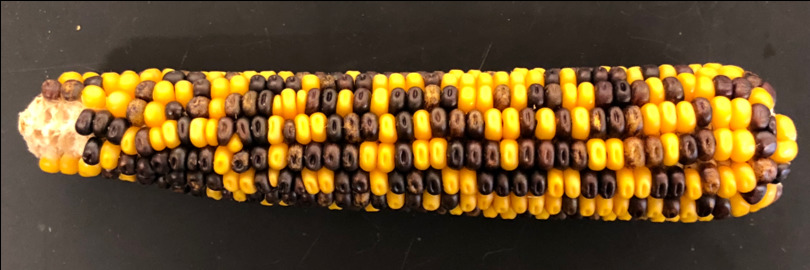
\includegraphics{./figures/mendel/Monohybrid_cross.jpg}
\caption{Monohybrid cross}
\end{figure}

\hypertarget{experimental-procedures}{%
\subsubsection{Experimental procedures}\label{experimental-procedures}}

\begin{enumerate}
\def\labelenumi{\arabic{enumi}.}
\tightlist
\item
  Count the number of purple and yellow kernels on one row of the F2 ear
  without removing the kernels.
\item
  Determine the ratio of purple to yellow.
\item
  Now tabulate the numbers obtained by each of your class mates in Table
  @ref(tab:mono) and add these figures to get a total.
\item
  Using the total numbers, determine a ratio of purple to yellow.
\end{enumerate}

\begin{longtable}[]{@{}cccc@{}}
\caption{(\#tab:mono) Monohybrid cross.}\tabularnewline
\toprule
Row \# & purple & yellow & ratio\tabularnewline
\midrule
\endfirsthead
\toprule
Row \# & purple & yellow & ratio\tabularnewline
\midrule
\endhead
1 & & &\tabularnewline
2 & & &\tabularnewline
3 & & &\tabularnewline
4 & & &\tabularnewline
5 & & &\tabularnewline
6 & & &\tabularnewline
7 & & &\tabularnewline
8 & & &\tabularnewline
9 & & &\tabularnewline
Total & & &\tabularnewline
\bottomrule
\end{longtable}

\hypertarget{dihybrid-cross-experiment-2}{%
\subsection{Dihybrid cross (Experiment
2)}\label{dihybrid-cross-experiment-2}}

In the second experiment, we will study the result obtained from a
\href{https://en.wikipedia.org/wiki/Dihybrid_cross}{dihybrid cross}. A
dihybrid cross is a cross between two different lines (varieties,
strains) that differ in two observed traits. In the name ``Dihybrid
cross'', the ``di'' indicates that there are two traits involved (in our
example designated R and Su), the ``hybrid'' means that each trait has
two different alleles (in our example R and r, or Su and su), and
``cross'' means that there are two individuals who are combining or
``crossing'' their genetic information. In our example, a pure strain of
corn producing purple-starchy kernels (RR SuSu) is crossed with a pure
strain producing yellow-sweet (rr susu). The starchy seeds are smooth,
the sweet seeds are wrinkled. The resulting F1 ears all bear
purple-starchy (smooth) kernels. Plants that are heterozygous for two
traits are called dihybrids. When the F1 is self-pollinated, the
resulting F2 generation contains various combinations (Figure
@ref(fig:dihybrid)).

\begin{figure}
\centering
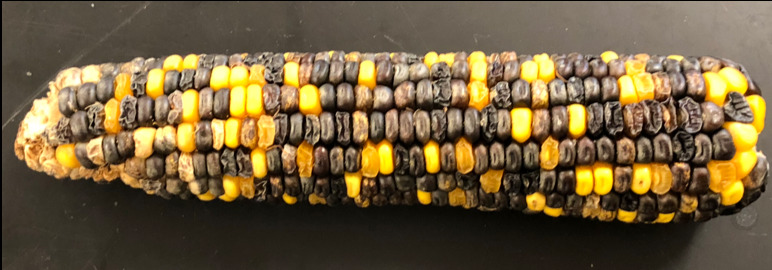
\includegraphics{./figures/mendel/Dihybrid_cross.jpg}
\caption{Dihybrid cross}
\end{figure}

The rules of meiosis, as they apply to the dihybrid, are codified in
Mendel's first law and Mendel's second law, which are also called the
Law of Segregation and the Law of Independent Assortment, respectively
(Table @ref(tab:mendel)). For genes on separate chromosomes, each allele
pair showed independent segregation. If the first filial generation (F1
generation) produces four identical offspring, the second filial
generation, which occurs by crossing the members of the first filial
generation, shows a phenotypic (appearance) ratio of \textbf{9:3:3:1},
where:

\begin{itemize}
\tightlist
\item
  the \textbf{9} represents the proportion of individuals displaying
  both dominant traits
\item
  the first \textbf{3} represents the individuals displaying the first
  dominant trait and the second recessive trait
\item
  the second \textbf{3} represents those displaying the first recessive
  trait and second dominant trait
\item
  the \textbf{1} represents the homozygous, displaying both recessive
  traits.
\end{itemize}

\hypertarget{experimental-procedures-1}{%
\subsubsection{Experimental
procedures}\label{experimental-procedures-1}}

\begin{enumerate}
\def\labelenumi{\arabic{enumi}.}
\tightlist
\item
  Carefully count the number of kernels of each phenotype appearing on a
  row of F2 ear. Tabulate the results and determine the totals and total
  ratios in Table @ref(tab:di).
\end{enumerate}

\begin{longtable}[]{@{}clllll@{}}
\caption{(\#tab:di) Dihybrid cross.}\tabularnewline
\toprule
\begin{minipage}[b]{0.04\columnwidth}\centering
Row \#\strut
\end{minipage} & \begin{minipage}[b]{0.19\columnwidth}\raggedright
purple and starchy (smooth)\strut
\end{minipage} & \begin{minipage}[b]{0.19\columnwidth}\raggedright
purple and sweet (wrinkled)\strut
\end{minipage} & \begin{minipage}[b]{0.19\columnwidth}\raggedright
yellow and starchy (smooth)\strut
\end{minipage} & \begin{minipage}[b]{0.19\columnwidth}\raggedright
yellow and sweet (wrinkled)\strut
\end{minipage} & \begin{minipage}[b]{0.03\columnwidth}\raggedright
ratio\strut
\end{minipage}\tabularnewline
\midrule
\endfirsthead
\toprule
\begin{minipage}[b]{0.04\columnwidth}\centering
Row \#\strut
\end{minipage} & \begin{minipage}[b]{0.19\columnwidth}\raggedright
purple and starchy (smooth)\strut
\end{minipage} & \begin{minipage}[b]{0.19\columnwidth}\raggedright
purple and sweet (wrinkled)\strut
\end{minipage} & \begin{minipage}[b]{0.19\columnwidth}\raggedright
yellow and starchy (smooth)\strut
\end{minipage} & \begin{minipage}[b]{0.19\columnwidth}\raggedright
yellow and sweet (wrinkled)\strut
\end{minipage} & \begin{minipage}[b]{0.03\columnwidth}\raggedright
ratio\strut
\end{minipage}\tabularnewline
\midrule
\endhead
\begin{minipage}[t]{0.04\columnwidth}\centering
1\strut
\end{minipage} & \begin{minipage}[t]{0.19\columnwidth}\raggedright
\strut
\end{minipage} & \begin{minipage}[t]{0.19\columnwidth}\raggedright
\strut
\end{minipage} & \begin{minipage}[t]{0.19\columnwidth}\raggedright
\strut
\end{minipage} & \begin{minipage}[t]{0.19\columnwidth}\raggedright
\strut
\end{minipage} & \begin{minipage}[t]{0.03\columnwidth}\raggedright
\strut
\end{minipage}\tabularnewline
\begin{minipage}[t]{0.04\columnwidth}\centering
2\strut
\end{minipage} & \begin{minipage}[t]{0.19\columnwidth}\raggedright
\strut
\end{minipage} & \begin{minipage}[t]{0.19\columnwidth}\raggedright
\strut
\end{minipage} & \begin{minipage}[t]{0.19\columnwidth}\raggedright
\strut
\end{minipage} & \begin{minipage}[t]{0.19\columnwidth}\raggedright
\strut
\end{minipage} & \begin{minipage}[t]{0.03\columnwidth}\raggedright
\strut
\end{minipage}\tabularnewline
\begin{minipage}[t]{0.04\columnwidth}\centering
3\strut
\end{minipage} & \begin{minipage}[t]{0.19\columnwidth}\raggedright
\strut
\end{minipage} & \begin{minipage}[t]{0.19\columnwidth}\raggedright
\strut
\end{minipage} & \begin{minipage}[t]{0.19\columnwidth}\raggedright
\strut
\end{minipage} & \begin{minipage}[t]{0.19\columnwidth}\raggedright
\strut
\end{minipage} & \begin{minipage}[t]{0.03\columnwidth}\raggedright
\strut
\end{minipage}\tabularnewline
\begin{minipage}[t]{0.04\columnwidth}\centering
4\strut
\end{minipage} & \begin{minipage}[t]{0.19\columnwidth}\raggedright
\strut
\end{minipage} & \begin{minipage}[t]{0.19\columnwidth}\raggedright
\strut
\end{minipage} & \begin{minipage}[t]{0.19\columnwidth}\raggedright
\strut
\end{minipage} & \begin{minipage}[t]{0.19\columnwidth}\raggedright
\strut
\end{minipage} & \begin{minipage}[t]{0.03\columnwidth}\raggedright
\strut
\end{minipage}\tabularnewline
\begin{minipage}[t]{0.04\columnwidth}\centering
5\strut
\end{minipage} & \begin{minipage}[t]{0.19\columnwidth}\raggedright
\strut
\end{minipage} & \begin{minipage}[t]{0.19\columnwidth}\raggedright
\strut
\end{minipage} & \begin{minipage}[t]{0.19\columnwidth}\raggedright
\strut
\end{minipage} & \begin{minipage}[t]{0.19\columnwidth}\raggedright
\strut
\end{minipage} & \begin{minipage}[t]{0.03\columnwidth}\raggedright
\strut
\end{minipage}\tabularnewline
\begin{minipage}[t]{0.04\columnwidth}\centering
6\strut
\end{minipage} & \begin{minipage}[t]{0.19\columnwidth}\raggedright
\strut
\end{minipage} & \begin{minipage}[t]{0.19\columnwidth}\raggedright
\strut
\end{minipage} & \begin{minipage}[t]{0.19\columnwidth}\raggedright
\strut
\end{minipage} & \begin{minipage}[t]{0.19\columnwidth}\raggedright
\strut
\end{minipage} & \begin{minipage}[t]{0.03\columnwidth}\raggedright
\strut
\end{minipage}\tabularnewline
\begin{minipage}[t]{0.04\columnwidth}\centering
7\strut
\end{minipage} & \begin{minipage}[t]{0.19\columnwidth}\raggedright
\strut
\end{minipage} & \begin{minipage}[t]{0.19\columnwidth}\raggedright
\strut
\end{minipage} & \begin{minipage}[t]{0.19\columnwidth}\raggedright
\strut
\end{minipage} & \begin{minipage}[t]{0.19\columnwidth}\raggedright
\strut
\end{minipage} & \begin{minipage}[t]{0.03\columnwidth}\raggedright
\strut
\end{minipage}\tabularnewline
\begin{minipage}[t]{0.04\columnwidth}\centering
8\strut
\end{minipage} & \begin{minipage}[t]{0.19\columnwidth}\raggedright
\strut
\end{minipage} & \begin{minipage}[t]{0.19\columnwidth}\raggedright
\strut
\end{minipage} & \begin{minipage}[t]{0.19\columnwidth}\raggedright
\strut
\end{minipage} & \begin{minipage}[t]{0.19\columnwidth}\raggedright
\strut
\end{minipage} & \begin{minipage}[t]{0.03\columnwidth}\raggedright
\strut
\end{minipage}\tabularnewline
\begin{minipage}[t]{0.04\columnwidth}\centering
9\strut
\end{minipage} & \begin{minipage}[t]{0.19\columnwidth}\raggedright
\strut
\end{minipage} & \begin{minipage}[t]{0.19\columnwidth}\raggedright
\strut
\end{minipage} & \begin{minipage}[t]{0.19\columnwidth}\raggedright
\strut
\end{minipage} & \begin{minipage}[t]{0.19\columnwidth}\raggedright
\strut
\end{minipage} & \begin{minipage}[t]{0.03\columnwidth}\raggedright
\strut
\end{minipage}\tabularnewline
\begin{minipage}[t]{0.04\columnwidth}\centering
Total\strut
\end{minipage} & \begin{minipage}[t]{0.19\columnwidth}\raggedright
\strut
\end{minipage} & \begin{minipage}[t]{0.19\columnwidth}\raggedright
\strut
\end{minipage} & \begin{minipage}[t]{0.19\columnwidth}\raggedright
\strut
\end{minipage} & \begin{minipage}[t]{0.19\columnwidth}\raggedright
\strut
\end{minipage} & \begin{minipage}[t]{0.03\columnwidth}\raggedright
\strut
\end{minipage}\tabularnewline
\bottomrule
\end{longtable}

\hypertarget{review-questions}{%
\subsection{Review Questions}\label{review-questions}}

\begin{enumerate}
\def\labelenumi{\arabic{enumi}.}
\tightlist
\item
  What is a gene?
\item
  What is an allele?
\item
  What are dominant and recessive alleles?
\item
  What is the genotype of an organism?
\item
  What is a trait?
\item
  What is the phenotype of an organism?
\item
  What is the genotype of the F1 generation of the monohybrid cross?
\item
  What is the phenotype of the F1 generation monohybrid cross?
\item
  What are the possible maternal and paternal genotypes of the F1
  gametes monohybrid cross?
\item
  What is the genotype of the parents of the dihybrid cross?
\item
  What are the phenotypes of the parents of the dihybrid cross?
\item
  What are the possible genotypes of the parent gametes of the dihybrid
  cross?
\item
  What is the genotype of the F1 generation of the dihybrid cross?
\item
  What is the phenotype of the F1 generation dihybrid cross?
\item
  What are the possible maternal and paternal genotypes of the F1
  gametes dihybrid cross?
\end{enumerate}


\end{document}
